\documentclass[main.tex]{subfiles}
\begin{document}

\marginpar{Wednesday\\ 2020-10-7, \\ compiled \\ \today}

% 243605

``Schwarzschild'' means ``Black Shield'': no relation though, it is the name of a German scientist. 
We have discussed the properties of this metric. 

Now, let us consider \textbf{geodesic motion} in the vacuum Schwarzschild spacetime. 

We cannot choose an arbitrary radius for an orbit around a Black Hole: there is an Innermost Stable Circular Orbit, and this has a direct impact on the accretion efficiency. 

We will use Latin letters for spacetime indices.
The four-velocity, as usual, is \(u^{i} = \dv*{x^{i}}{\tau }\), where \(\dd{\tau }\) is the proper time. 
Also, for massive particles we also have the four-momentum \(p^{i} = m u^{i}\). 

Analogously to classical mechanics, the Lagrangian of a free particle is 
%
\begin{align}
L =- \sqrt{- g_{ij} p^{i} p^{j}} = -m \sqrt{- g_{ij} u^{i} u^{j}}
\,,
\end{align}
%
and the corresponding Euler-Lagrange equations read 
%
\begin{align}
\dv{}{\tau } \qty(\pdv{L}{u^{i}}) - \pdv{L}{x^{i}} = 0
\,,
\end{align}
%
however we will not study these in the general case, it is too complicated. 
It can be shown that along a geodesic the Lagrangian itself is conserved: \(L = \const\). 
Therefore, \(g_{ij} u^{i} u^{j}\) is also a constant, a negative one since the velocity is timelike. We can then set it to \(-1\) by reparametrizing, so we will have \(u^2 = -1\) and \(p^2= -m^2\). 

Suppose that the there is a certain coordinate \(x^{k}\) such that 
%
\begin{align}
\pdv{g_{ij}}{x^{k}} = 0
\,,
\end{align}
%
that is, the metric does not change along the \(x^{k}\) direction. This is known as a \textbf{Killing vector} for the metric.
Therefore, 
%
\begin{align}
\pdv{L}{x^{k}} =0
\,,
\end{align}
%
which tells us that 
%
\begin{align}
\dv{}{\tau } \qty(\pdv{L}{ u^{k}}) = 0
\,,
\end{align}
%
meaning that this cyclic variable gives us a conserved quantity. If we do the calculation, the constant comes out to be
%
\begin{align}
m g_{kj} u^{j} = p_k =  \const
\,.
\end{align}

This is the case in Schwarzschild spacetime: the metric only depends on \(r\) and \(\theta \), while \(t\) and \(\varphi \) are cyclic. 
Therefore, we will have two constants of motion: in terms of the momentum, \(p_t\) and \(p_{\varphi }\). 

We can denote them as \(E = - p_t\) and \(L = p_\varphi \). 
Let us start from \(L\):
%
\begin{align}
L &= g_{\varphi k} p^{k} = g_{\varphi \varphi } m \dv{x^{\varphi }}{\tau }  \\
&= r^2 \sin^2 \theta m \dv{\varphi }{\tau } \\
\dv{\varphi }{\tau } &= \frac{L}{m r^2 \sin^2 \theta }
\,.
\end{align}

Now, geodesic motion is in general planar since the metric is spherically symmetric: we do not lose any generality by setting \(\theta = \pi /2\), so we can simplify \(\sin^2 \theta = 1\).

In general, even in Netwonian mechanics, when discussing orbits we can decompose the velocity into the radial and perpendicular direction. 
The angular momentum, in classical Newtonian mechanics, has a modulus \( \abs{\vec{L}} = \abs{\vec{r} \wedge m \vec{v}} = mr v_\varphi = mr^2 \dot{\varphi} \). This is the same relation we have found here.  

The energy of an object with four-momentum \(p_k\) as measured by an observer with four-velocity \(u^{k}\) is given by \(E = - p_k u^{k}\). 
We choose an observer which is static with respect to the coordinates:\footnote{Its four velocity will be given by \(k^{i} = (1 / \sqrt{-g_{tt}}, \vec{0})\) by normalization.}
then, we have \(\dv*{t}{\tau } = \gamma / \sqrt{- g_{tt}} \), so
%
\begin{align}
E &= -g_{tt} m \dv{x^{t}}{\tau } = 
+ \qty(1 - \frac{2M}{r}) \frac{m}{\sqrt{1 - v^2}} \frac{1}{\sqrt{- g_{tt}}} \\ 
&= \sqrt{1 - \frac{2M}{r}} m \gamma 
 \\
&\approx m \qty(1 - \frac{M}{r} + \frac{v^2}{2})
\,
\end{align}
%
so in the Newtonian limit (\(M \ll r\), \(v \ll 1\)) this is regular expression for the conservation of energy, gravitational plus kinetic.

Now we have the tools to study geodesic motion: let us write down \(p^2 = -m^2\) explicitly, 
%
\begin{align}
g_{tt} \qty(p^{t})^2 + g_{rr} \qty(p^{r})^2 + \underbrace{g_{\theta \theta } \qty(p^{\theta })^2}_{= 0 \text{ if } \theta \equiv \pi /2} + g_{\varphi \varphi } \qty(p^{\varphi })^2 = - m^2
\,,
\end{align}
%
and if we substitute we must be careful: the constants of motion are related to the \emph{covariant} components of the quantities, so we have 
%
\begin{align}
g_{tt} \qty(g^{tt} p_t)^2 
+ g_{rr} \qty(g^{rr} p_r)^2
+ g_{\varphi \varphi } \qty(g^{\varphi \varphi } p_\varphi )^2
&= - m^2 \\
g_{tt} \qty(g^{tt})^2 E^2 
+ g_{rr} \qty(p^{r})^2
+ g_{\varphi \varphi } \qty(g^{\varphi \varphi })^2 L^2
&= - m^2 \\
 g^{tt} E^2 
+ g_{rr} \qty( p^r)^2
+ g^{\varphi \varphi } L^2
&= - m^2 \\
 -\qty(1 - \frac{2M}{r})^{-1} E^2 
+ \qty(1 - \frac{2M}{r})^{-1} \qty( p^r)^2
+ \frac{L^2}{r^2}
&= - m^2 \\
 -\qty(1 - \frac{2M}{r})^{-1} E^2 
+ \qty(1 - \frac{2M}{r})^{-1} m^2\qty(\dv{r}{\tau })^2
+ \frac{L^2}{r^2}
&= - m^2 
\,,
\end{align}
%
which is an ODE for the single function \(r (\tau )\): we can integrate this to find the shape of the trajectory. 
We now divide everything by \(m^2\), and define the specific energy and angular momentum \(\epsilon = E / m\) and \(\ell = L / m\): 
%
\begin{align}
\qty(1 - \frac{2M}{r})^{-1} \qty[\qty(\dv{r}{\tau })^2 - \epsilon^2]
+ \frac{\ell^2}{r^2} = -1
\,.
\end{align}

We can then express this as 
%
\begin{align}
\qty(\dv{r}{\tau })^2 = - \qty(1 + \frac{\ell^2}{r^2}) \qty(1 - \frac{2M}{r}) + \epsilon^2
\,,
\end{align}
%
which can give us \(r(\tau )\) or \(r(\varphi )\) in a rather simple way numerically, however the answer is not analytic: it is given by an elliptic integral. 

We can study it analytically by looking at the turning points, those with \(\dv{r}{\tau } = 0\).
These will tell us about the shape of the orbit. 
They obey the equation 
%
\begin{align}
0 = - \qty(1 + \frac{\ell^2}{r^2}) \qty(1 - \frac{2M}{r}) + \epsilon^2
\,,
\end{align}
%
which means 
%
\begin{align}
\frac{\ell^2}{r^2} = \qty(\epsilon^2 -1 + \frac{2M}{r}) \qty(1 - \frac{2M}{r})^{-1}
\,,
\end{align}
%
which has the solutions 
%
\begin{align}
\ell_{\pm} = \pm r \qty[ \qty(\epsilon^2 - 1 + \frac{2M}{r}) \qty(1 - \frac{2M}{r})^{-1}]^{1/2}
\,.
\end{align}

Let us define \(\lambda = \ell / 2M\) and \(x = r / 2M\). These are dimensionless in our units. Also, we define \(\Gamma = \epsilon^2- 1\). They satisfy 
%
\begin{align}
\lambda_{\pm} 
= \pm x \sqrt{\qty(\Gamma + \frac{1}{x}) \qty(1 - \frac{1}{x})^{-1}}
= \pm x \sqrt{\frac{x\Gamma + 1}{x-1}}
\,.
\end{align}

We want to draw these as curves in the  \(x\), \(\lambda \) plane. 
We fix a value of \(\ell\), which means we have chosen \(\lambda \). This depends on the initial conditions of the motion of the particle. 
If this \(\lambda \) is a \(\lambda _+\), then \(x\) can move in all the region \(x(\lambda _+)  < x < \infty \).

This is the relativistic analog of the hyperbolic trajectories in the Keplerian case. 

Let us try to compute \(\dv{\lambda_{\pm}}{x}\): this yields 
%
\begin{align}
2 x^2 \Gamma + 3 x - 3 x \Gamma - 2 &= 0 \\
\Gamma \qty(2 x^2 - 3x) + x-2 &= 0  \\
\Gamma &= \frac{2-x}{2 x^2 - 3x}
\,.
\end{align}

This means we have a single curve, which will relate \(\Gamma \) and \(x\). 
The physical cases are only the ones with \(\Gamma > -1\). 
The minimum is at \(x = 3\), corresponding to \(r = 6M\), where we have \(\Gamma = - 1 /9\). This corresponds to \(\epsilon^2 - 1\): so, \(\epsilon = \sqrt{2} \times 2/3 \).

For \(- 1/9 < \Gamma < 0\) we have two choices for \(x\), for \(\Gamma > 0\) we have only one. 

Coming back to the \(\lambda_{\pm}\) curves, we can have \(\lambda_{\pm}\) as two distinct curves, and there is a region around \(\lambda = 0\) for which the particle will cross the horizon. 

This allows us to compute the cross-section for gravitational capture, which is nonvanishing \emph{even if} we neglect the size of the black hole. 

\begin{figure}[ht]
\centering
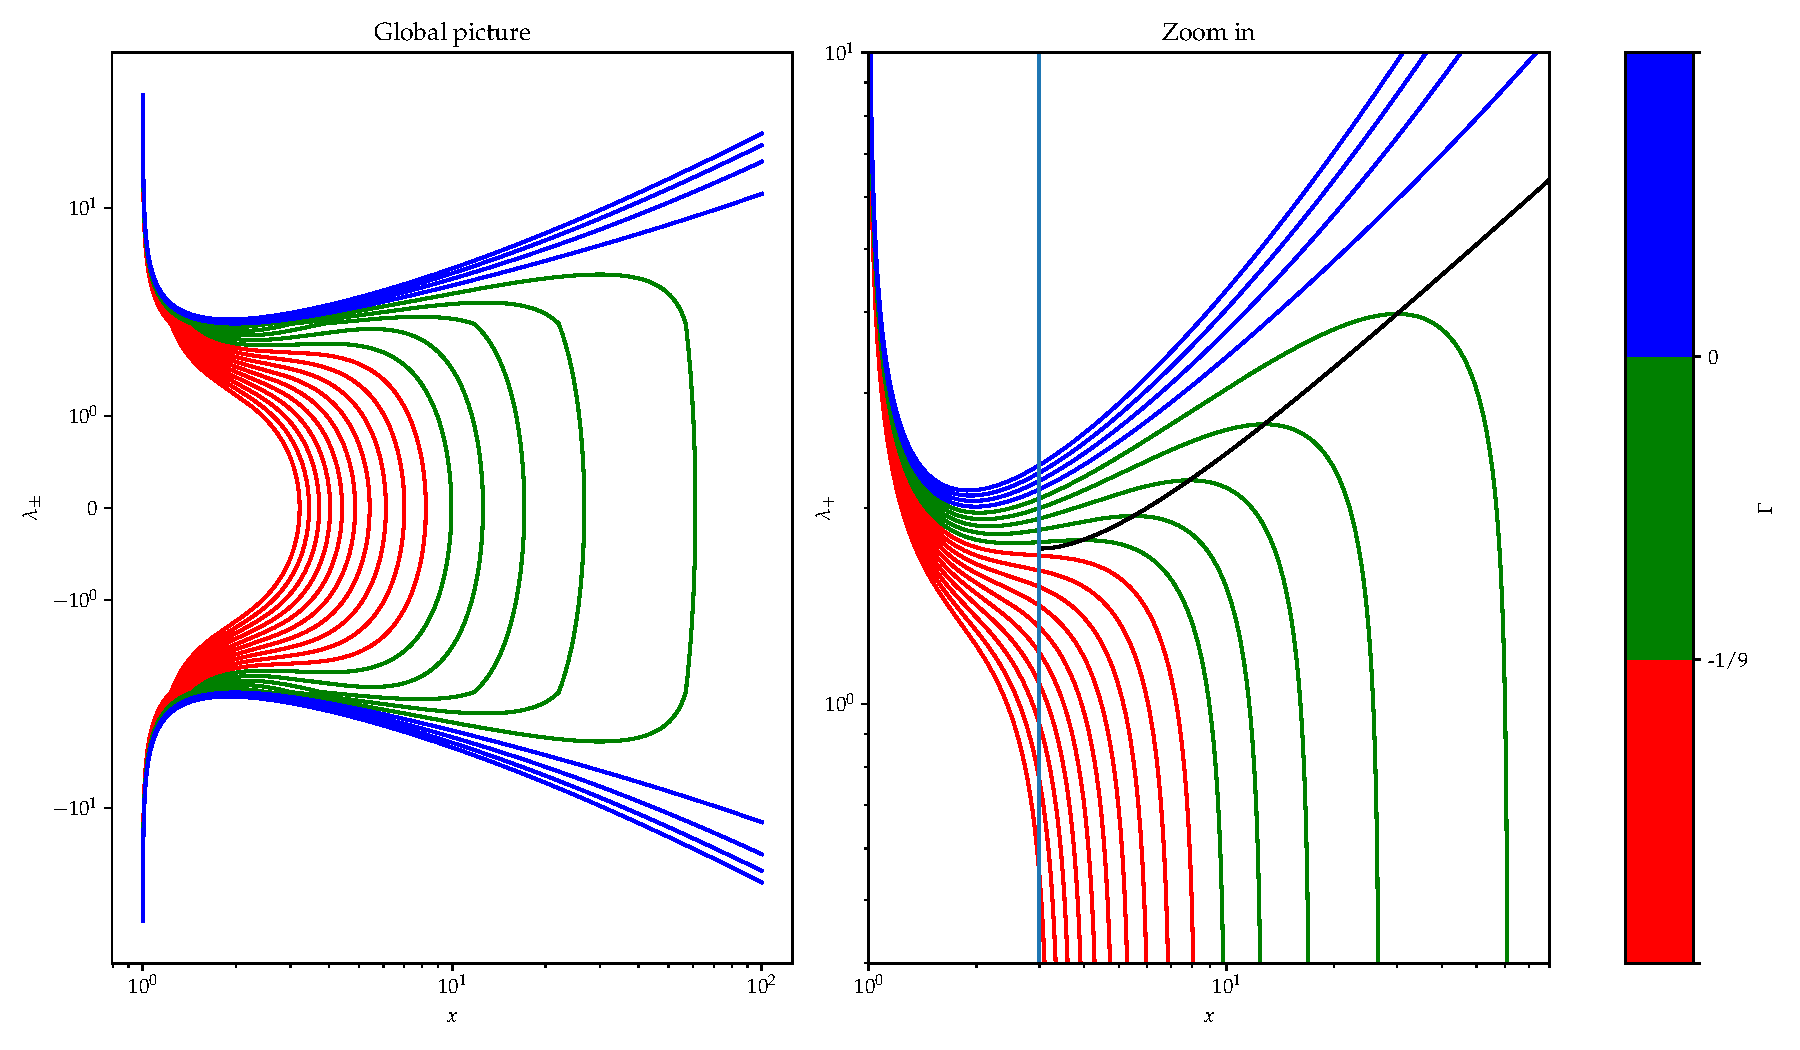
\includegraphics[width=\textwidth]{figures/schwarzschild_orbit_inversions.pdf}
\caption{Inversion points for orbits in the Schwarzschild exterior metric. The vertical line in the zoomed-in view marks \(x =3\), or \(r = 6M\).}
\label{fig:schwarzschild-inversion}
\end{figure}

\end{document}
